%نام و نام خانوادگی:
%شماره دانشجویی: 
\مسئله{LALR یا SLR!}

\پاسخ{اثبات به برهان خلف.
فرض خلف : slr(1) بدون conflict داریم اما مق(1) بدون conflict  نداریم. از آنجایی که در lalr1 برخورد داشته ایم پس یک terminal وجود دارد که در آنجا هم می‌توانیم کاهش دهیم هم شیفت دهیم. پس یک قاعده تولید وجود دارد که terminal ذکر شده در بالا در سمت راست nonterminalفرضی وجود دارد پس این nonterminal در فالو خود terminal ذکر شده را دارد. پس در slr1 هم conflictداریم. تناقض.

حال می‌خواهیم مثالی بزنیم که در SLR1 برخورد دارد ولی درLalr1 ندارد

\lr{
\\E -> S
\\E -> a + b + S + c
\\S -> A + B
\\B -> B + c
\\A -> g
\\Follow E = \$
\\Follow S = \$ , +
\\Follow B = + , \$
\\Follow A = not important
\\
}
ابتدا نمودار \lr{SLR1} را می‌ کشیم و نشان می‌دهیم در آن برخورد داریم

\begin{figure}[H]
			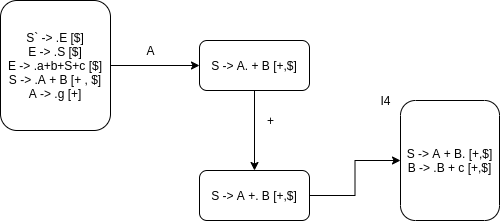
\includegraphics[width=\linewidth]{./commons/Q7.png}
			\label{fig:Q7}
		\end{figure}
		
همانطور که مشاهده می‌کنید در stateشماره 4 هم می‌توانیم در + عمل کاهش را انجام دهیم چون در فالو S  آمده هم می‌توانیم با + عمل شیفت را انجام دهیم و از آن خارج شویم
حال دیاگرام lr1را رسم می‌کنیم.
\begin{figure}[H]
			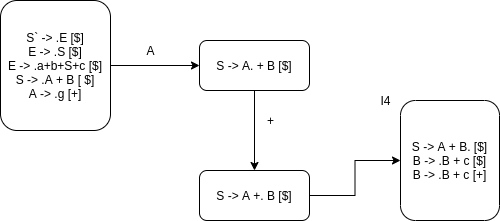
\includegraphics[width=\linewidth]{./commons/Q72.png}
			\label{fig:Q72}
		\end{figure}
		مشاهده می‌کنیم که در state شماره 4 در \$ عمل کاهش را انجام می‌دهیم و با + میتوانیم خارج شویم در نتیجه برخورد ندارند
}